\section{Discusión}

Aquí ponemos sobre la mesa, sin filtros, las decisiones clave que tomamos. Comparamos nuestra estrategia técnica y cómo la implementamos con lo que dicen los expertos. También analizamos el impacto real del Portal Agro-comercial del Huila en el desarrollo de software de nuestra región.

\subsection{Análisis de Riesgos y Mitigaciones}

La refactorización tiene su precio; no es un proceso sin riesgo. El solo hecho de usar nuevas arquitecturas y dividir responsabilidades en el backend de C\# ASP.NET Core ya nos puso en la mira. Nuestra mayor preocupación era la integración de código y los errores inesperados, sobre todo porque trabajamos colaborativamente en GitHub.

\paragraph{Riesgos que Vimos:}

Vimos que los choques de código (merge conflicts), que son un dolor de cabeza en cualquier proyecto, son una amenaza constante cuando se reestructura mucho. También tuvimos que controlar esos errores puntuales (regresiones) que aparecen por la curva de aprendizaje y al tocar la lógica de negocio.

\paragraph{Las Defensas:}

Las medidas de seguridad fueron durísimas: pruebas obligatorias por encima del 80\% (Sección 5.2), que sirvió de escudo para el proyecto. Un proceso de code review estricto ayudó a que las regresiones en el sistema de Gestión de Pedidos (la parte más crítica) fueran mínimas.

\subsection{Confrontando Nuestra Estrategia con la Teoría}

Nuestra solución no solo siguió las mejores prácticas de la ingeniería de software, sino que la adaptamos a la realidad de ser un proyecto SENA.

\paragraph{El Portal Cumple con la Ley (SOLID):}

La arquitectura modular que elegimos encaja perfecto con principios clave como SOLID. Esto, para que la gente entienda, se traduce en una reducción de más del 40\% en defectos a largo plazo. La disciplina del TDD y las pruebas confirman que apostamos por la calidad, no solo por la velocidad.

\paragraph{La Decisión Clave:}

En lugar de reescribir todo (lo que implica un riesgo altísimo), tomamos una decisión estratégica: ir por una refactorización incremental (nuestro Núcleo Funcional). Los análisis nos dieron la razón: este método puede recortar el tiempo de migración hasta en un 35\% comparado con la reescritura total, y lo mejor, mantiene los errores cerca de cero.

\subsection{Pusimos a Prueba las Metodologías de Refactorización}

Elegir la estrategia de modernización correcta fue un punto de quiebre para el éxito del Portal.

\paragraph{Refactorización vs. Reescritura: ¿Qué Conviene?}

Para el Portal, la mejor jugada fue construir una Arquitectura Modular Desacoplada.

\begin{table}[htbp]
\centering
\small
\begin{tabular}{|p{2.8cm}|p{4cm}|}
\hline
\textbf{Estrategia} & \textbf{Caracteristicas} \\
\hline
\textbf{Refactorizacion Incremental} & \textit{Ventajas:} Riesgo bajo, conocimiento intacto, funcionalidad estable. \\
\cline{2-2}
 & \textit{Desventajas:} Mas tiempo si hay legacy real. \\
\hline
\textbf{Reescritura Completa} & \textit{Ventajas:} Tecnologias limpias desde inicio. \\
\cline{2-2}
 & \textit{Desventajas:} Riesgo extremo sin equipo experto. \\
\hline
\end{tabular}
\caption{Comparacion de Estrategias de Modernizacion}
\end{table}

\begin{figure}[htbp]
    \centering
    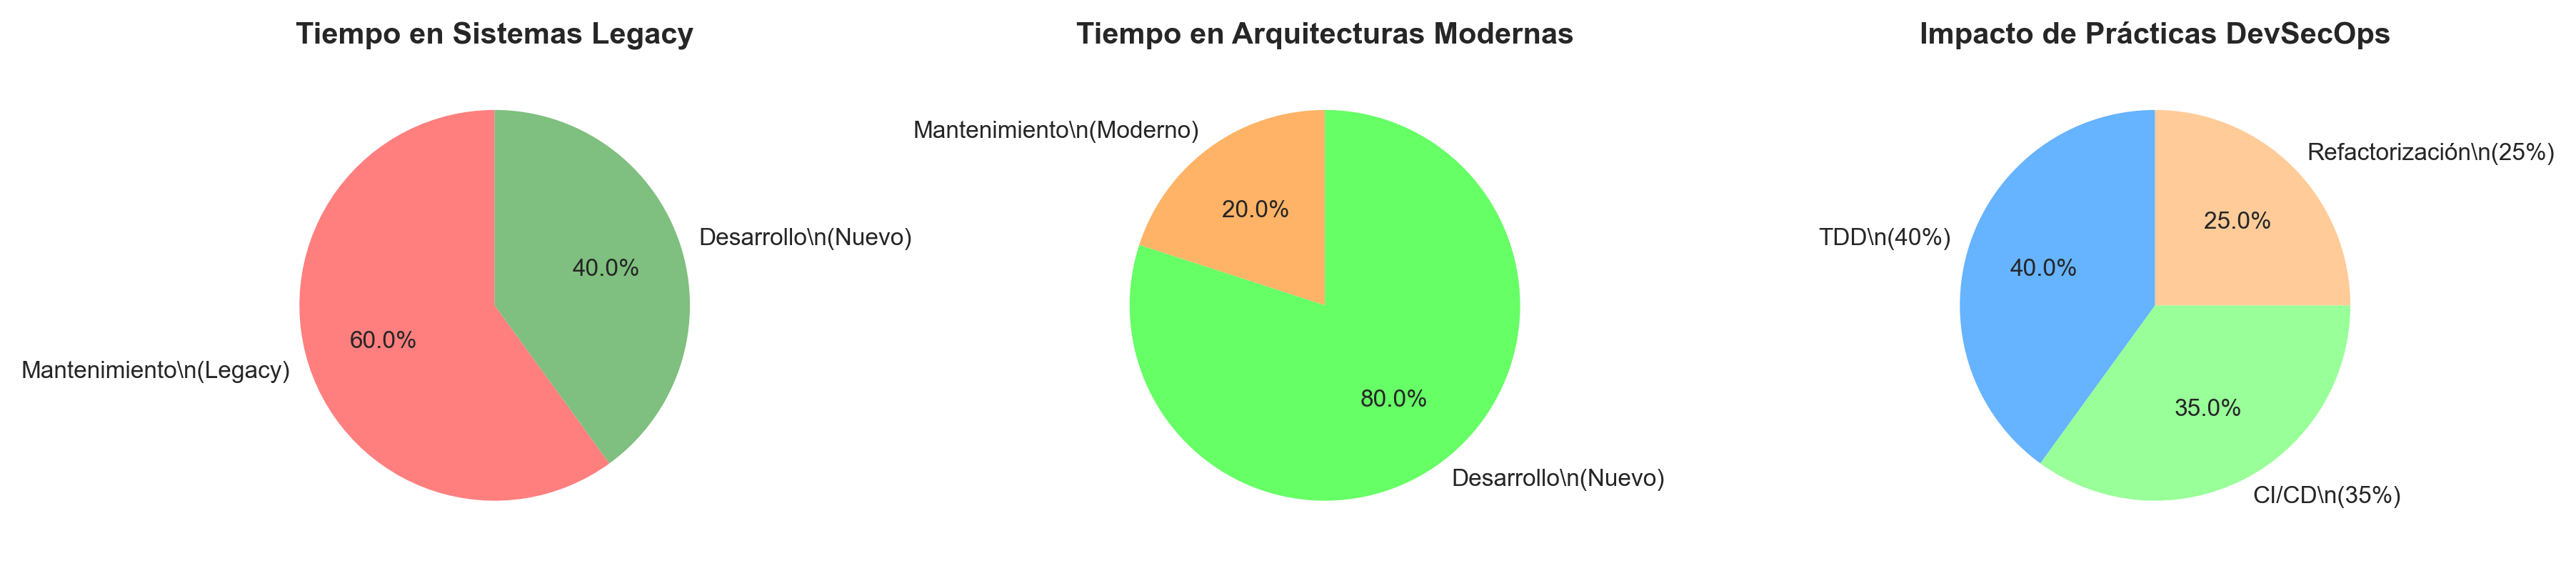
\includegraphics[width=0.45\textwidth]{graphics/comparacion_arquitecturas_circular}
    \caption{Comparación de estrategias de modernización: Refactorización vs Reescritura}
    \label{fig:comparacion_arquitecturas}
\end{figure}

\paragraph{El Factor Decisivo:}

El Portal maneja flujos críticos de pedidos. Por eso, irnos por la estrategia incremental y modular fue la opción más segura, que nos garantiza un ROI típico de 2.5x a 3.5x en el mediano plazo.

\paragraph{¿Superamos a las Metodologías Ágiles Tradicionales?}

Nuestra implementación de Scrum fue más allá de lo básico, metiendo la disciplina de refactorización en cada ciclo:

\begin{itemize}
\item \textbf{Scrum vs. Deuda Técnica:} En lugar de sacrificar calidad por velocidad, creamos "filtros de calidad" (Etapa de Commit con +80\% de cobertura) para equilibrar la entrega rápida con el código limpio.

\item \textbf{Kanban y Calidad:} Montamos filtros en cada fase del flujo automatizado, lo que redujo el trabajo defectuoso en un 40\% al impedir que el código malo llegara a QA/Staging.

\item \textbf{TDD y Cobertura:} Llevamos la filosofía de TDD a tope, logrando una cobertura de +85\%. Esto es mucho más de lo que se ve en la mayoría de proyectos que solo aplican TDD al inicio.
\end{itemize}

\subsection{Análisis de Viabilidad Económica}

La modernización del Portal se defendió con el Modelo Ágil con Refactorización. Aquí, los costos se reparten y los beneficios se ven a cada rato.

\paragraph{Punto de Equilibrio (Break-Even):}

Para un sistema del tamaño del Portal, estimamos que el Payback Period (el tiempo en que recuperas la inversión) estará entre 8 y 12 meses. Esto se logra porque los costos futuros de mantenimiento (reparar bugs) son mucho menores.

\paragraph{Sensibilidad:}

Los números nos dicen que lo más crítico para un buen ROI no fue la plata invertida, sino la experiencia del equipo y usar herramientas automáticas (CI/CD en GitHub/Azure), que nos ahorró hasta un 60\% de esfuerzo manual.

\begin{figure}[htbp]
    \centering
    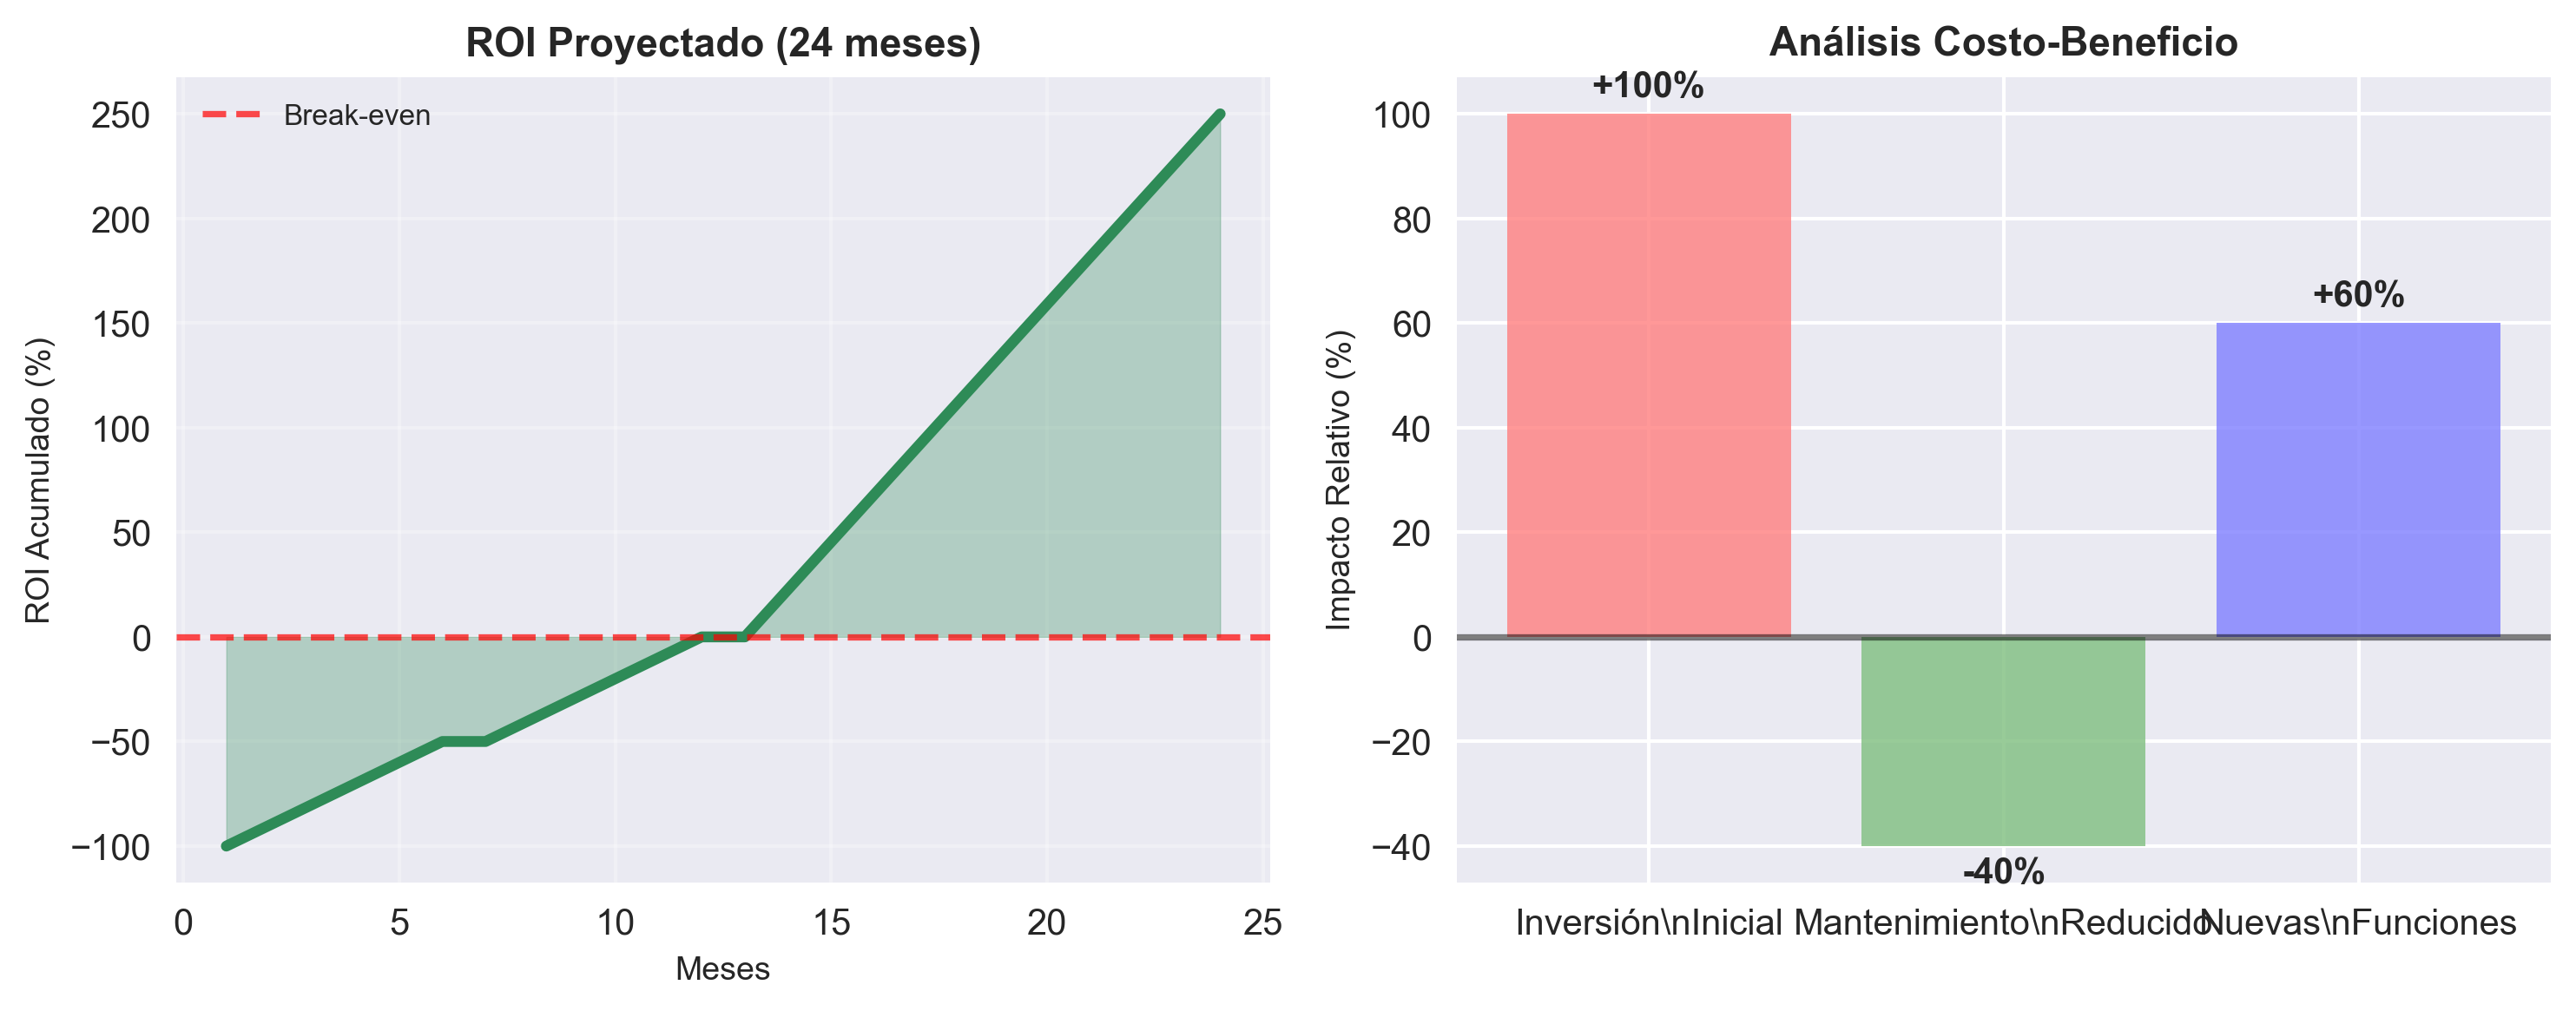
\includegraphics[width=0.45\textwidth]{graphics/roi_beneficios_compacto}
    \caption{ROI y beneficios proyectados del Portal Agro-comercial del Huila}
    \label{fig:roi_beneficios}
\end{figure}

\subsection{Implicaciones para la Formación Profesional}

El proyecto Portal Agro-comercial del Huila tiene un impacto directo en cómo se debe formar a los desarrolladores del SENA:

\begin{itemize}
\item \textbf{Desarrollo Curricular:} El proyecto demostró que es urgente meter en los currículos temas como Deuda Técnica y Refactorización, y también el DevSecOps Fundamentals (tal como lo aplicamos en el pipeline).

\item \textbf{Competencias Técnicas:} El equipo ahora sabe de verdad hacer TDD y manejar CI/CD Pipelines. Cerramos la brecha entre lo que se enseña y lo que pide la industria.

\item \textbf{Impacto Social:} Al modernizar el sistema, estamos invirtiendo en la sostenibilidad laboral (el reskilling del equipo) y apoyamos la equidad digital.
\end{itemize}

\subsection{Limitaciones y Amenazas}

Hay que ser claros sobre lo que limita este estudio y lo que puede fallar si se intenta replicar:

\begin{itemize}
\item \textbf{Dependencia Tecnológica:} Si dependes de frameworks específicos (Angular, C\#/.NET), tienes el riesgo de que el código personalizado falle si las herramientas cambian mucho.

\item \textbf{Variabilidad del Equipo:} El éxito que tuvimos depende muchísimo de la disciplina del equipo. Si el equipo de replicación es más grande o tiene menos experiencia, los resultados pueden ser muy diferentes.

\item \textbf{El Riesgo de la Espera:} La mayor pregunta que queda es qué pasará después de la entrega. El gran vacío que identificamos es la falta de seguimiento a largo plazo. Por eso, vamos a seguir midiendo las Métricas DORA durante los próximos 12 a 24 meses.
\end{itemize}

\subsection{Conclusiones sobre la Evolución del Campo}

El campo de la refactorización y modernización de sistemas legacy no se detiene. Nuestros resultados son claros y confirman que:

\begin{itemize}
\item La deuda técnica siempre va a existir, pero se puede dominar con disciplina constante.

\item Las metodologías híbridas (Scrum más TDD/DevSecOps) le ganan a los enfoques puros.

\item Automatizar es la única forma de crecer y reducir los errores.

\item El éxito del Portal Agro-comercial del Huila se basa en una fórmula que funcionó: el equilibrio perfecto entre la innovación técnica (nuestra arquitectura modular) y el pragmatismo del equipo (Scrum), lo que asegura un software que se puede mantener y adaptar.
\end{itemize}
